\documentclass[main.tex]{subfiles}

\begin{document}

\section{\gama} \label{chapter:gama}

The \acf{GAMA} is a framework to aid computational scientists in the development or porting of data-parallel applications to heterogeneous computing platforms. Currently \hetplat support includes only systems composed of \textit{x86-64} \cpu cores and one or more CUDA-enabled \gpu devices.

\gama provides an abstraction of the hardware platform, attempting to free the programmer from the workload scheduling and data movement issues across the different resources. In \gama, an application is composed of a collection of jobs, each defined as a set of tasks applied to a different input data set. Every job shares the same global address space, instead of directly using the private memory of each device.

One of the main focuses of \gama is to efficiently execute irregular applications, which are particularly harder to make estimations on. In an irregular application, input data sets and their sizes cannot be used to make assumptions about how the task will perform under a similar, but not equal set of input. This does not hold true for regular applications, which is what makes their scheduling easier. As such, irregular applications can be more difficult to extract parallelism from, especially when workload is distributed, as is the case with \hetplats and their frameworks.


\subsection{Memory Model}

\gama uses an unified programming model that assumes a hierarchy composed of multiple devices (both \cpus and \gpus), where each device has access to a private address space (shared by all computing units, or cores, within that device), and a distributed memory system between devices. The framework assumes that multiple computing units of an individual device can cooperate and communicate through a shared memory space, and that the underlying programming and execution model of that device provides synchronization mechanisms (barriers, atomics and memory fences).
To abstract the distributed memory model that is used between devices, \gama introduces a global address space. \Cref{fig:gama_memory_model} illustrates how \gama understands the memory hierarchy of a \hetplat.


\subsubsection{Memory Consistency}

Communication between memory spaces of different devices is expensive due to the need of synchronization and data transfers between the host \cpu and the devices. Due to this, a relaxed consistency model is used, which enables the system to optimize data movements between devices, offering the developer a single synchronization primitive to enforce memory consistency.

\subsubsection{Software Cache}

Some applications require safe exclusive access to specific partitions of a data set. To address this issue, a software cache shared between devices was implemented. This ensures that the required data is as close to the device as possible, taking advantage of the local memory of each device. It also provides a safeguard mechanism in combination with the global memory system, to ensure that each device has a copy of a specific partition, when requested by the application. Additionally, the cache local copies on the device shared memory space use semantically correct synchronization primitives within the device.

\begin{figure}[!htp]
  \centering
  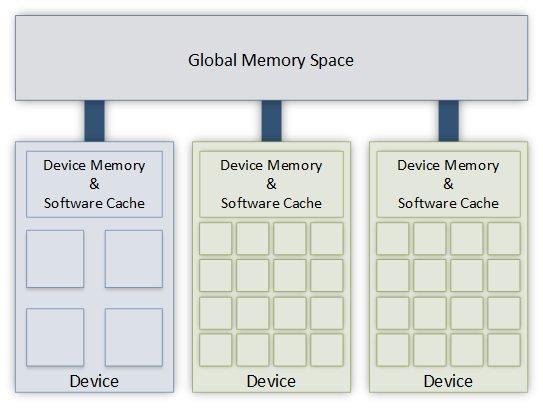
\includegraphics[width=0.6\textwidth]{visio/gama}
  \caption[\gama memory model]{\gama memory model, an extension to the one shown in \cref{fig:hetplat} \label{fig:gama_memory_model}}
\end{figure}

\subsection{Programming and Execution Model}

To better understand the programming and execution model employed in \gama, some key concepts must be introduced:

\begin{description}
  \item[\acf{CU}] \hfill \\
    In \gama, a \acl{CU} is an individual execution unit, capable of executing a general-purpose application. In the context of a \cpu, a \acl{CU} represents a single core, while on a \gpu, in the current implementation represents a single \acf{SM}. Thus the terms \ac{CU} and \cpu-core may be used with the same meaning.

  \item[Device or Worker] \hfill \\
    Represents a collection of \aclp{CU} that share some level of memory (e.g.\ the CPU cores on the same machine, or the \sms  of a single \gpu).

  \item[Host] \hfill \\
    The group of all devices within a single computational node. Currently \gama supports only a single-host, taking advantage of multiple computational nodes. As such, the host represents the top-most hierarchy layer in \gama's execution model

  \item[Domain] \hfill \\
    A global view of a particular data structure that enables developers to access any memory location using the global address space, and hiding the complexity of the underlying memory system. At the application level, the user is able to define filters of partial views of a single domain, allowing the system to identify the required communication primitives and enforce the global address space, the memory consistency model, and cache and synchronization mechanisms.

  \item[Job] \hfill \\
    A tuple associating data domains with the corresponding computations related to it (the computational kernel), and a specialized dicing function that defines the best strategy for job granularity, recursively splitting the job into smaller tasks across the data domains. This dicing function is somewhat analogous to the ability of defining task granularity with tools such as \acs{OpenMP}, but it can employ more flexible solutions, to account for the irregularity of the algorithms.

  \item[Kernel] \hfill \\
    The computation associated with a job. In a best-case scenario, a computational kernel can be mapped directly to a given device simply with the help of the toolkit supporting that device. In most cases, however, the kernel needs to be tailored to a specific device's programming model. This is achievable by extending the job description with the addition of the specialized kernel for a specific device. This feature also enhances the programming model by enabling developers to tailor specific computational kernels for each platform, taking advantage of architecture-specific features.

\end{description}

The organization of the execution model between computing units, Devices and Hosts ensures that a consistent model can be implicitly assumed, where \acsp{CU} within the same device share a common address space, allowing the usage of device-specific synchronization mechanisms to manage the coordination of concurrent executions within that device.

An application in GAMA is a collection of jobs submitted to a run-time system for scheduling among the available computational resources. Dependencies among jobs can be specified with explicit synchronization barriers. The main goal of the runtime scheduler is to reduce the overall execution time of any given application.

\subsubsection{Scheduling} \label{sec:gama_sched}

The scheduler uses information provided by each job in order to determine the best scheduling policy, based on current runtime states, as well as execution history. If the granularity of a job is too coarse to enable a balanced scheduling policy, \gama will recursively employ the dicing function of a job to adjust the task granularity to the capabilities of the devices.

Internally, \gama uses a variant of the \ac{HEFT} scheduling algorithm \cite{topcuoglu2002performance}, which uses the computation and communication costs of each task, in order to assign every task to a device in such a way that minimizes the estimated finish time of the overall task pool. This variant of \acs{HEFT} instead attempts to make a decision every time it is applied to the task pool, so that tasks on the multiple devices take the shortest possible time to execute \cite{thesisMariano12}.


\subsection{The Polu Case-Study}

Preliminary tests of the \gama capabilities were performed in the early training stages, which included well studied cases, such as the SAXPY and the Barnes-Hut algorithms.

Later, an implementation of a small, first order finite volume method was implemented using \gama, using the previously implemented versions of that same algorithm for comparison references. These versions included a sequential implementation, and two parallel ones, one with \openmp, and another with \cuda. The details of the algorithm are described in more detail below.

The \texttt{polu} application, computes the spread of a material (e.g.\ a pollutant) in a bi-dimensional surface through the course of time. This surface is discretely represented as a mesh, composed mainly of edges and cells. The input data set contains data on the mesh description, the velocity vector for each cell and an initial pollution distribution.

\texttt{Polu} has already been the subject of a parallelization study in \cite{naps2012}, which described the incremental work where the application was improved from a sequential implementation, first through a process of analysis and sequential optimization, and then subject to parallelization using two techniques, a shared memory \cpu implementation with \openmp, and a \gpu implementation with \cuda.

\subsubsection{The Algorithm} \label{sec:polu:alg}

The \texttt{polu} algorithm is a first order finite volume method, where each mesh element only communicates directly with its first level neighbours in the mesh, a typical case of a stencil computation. The algorithm is very irregular in terms of memory access patterns, since the mesh input generator, \texttt{gmsh}, suffers from deep locality issues, turning memory accesses ordered by cells or edges close to random.

The execution of the algorithm consists of looping through two main kernels, advancing in time until an input-defined limit is reached. These two kernels are:
\begin{description}
\item[\texttt{compute\_flux}] \hfill \\
  In this step, a flux is calculated for each edge, based on the current pollution concentration of each of the adjacent cells. A constant value, the \textit{Dirichlet} condition, is used for the boundary edges of the mesh, replacing the value of the missing cell. This flux value represents the amount of pollution that travels across that edge in that time step.

\item[\texttt{update}] \hfill \\
  With the previously calculated fluxes, all cell values are updated, with each cell receiving contributions from all the adjacent edges. After this, one time step has passed.
\end{description}

\subsubsection{Implementation}

To run the algorithm using the framework, both kernels had to be re-written, following the \gama model of jobs. Data structures were also re-written to make use of the facilities provided by \gama to allow memory to be automatically handled by the global address space.
This presents an obviously large amount of development work, since almost everything had to be re-written according to the \gama rules. However, it has to be taken into account the fact that this additional work also had to be performed in the previous implementations studied in \cite{naps2012}, since most of the original code was not suitable for efficient parallelization.

From this, one initial consideration can already be made about the framework, in the sense that the effort required to parallelize an application following the \gama rules might be too high, if a given application was already written for a parallel environment. Since specific data structures and job definitions need to be used, this may hamper the adoption of \gama by already implemented solutions, unless the performance advantages are significant enough to justify the additional effort.

\subsubsection{Study limitations}

Several restrictions apply to the input generation for this algorithm. In particular, the utility required to generate a mesh with arbitrary resolution has an estimated complexity of $O(N^3)$, which prevented large enough test cases to be generated. The largest available input contained only around $400,000$ cells, and represented a total memory footprint of just over $40MB$, which is extremely small, and does not allow a good enough analysis on resource usage. With such a low resource occupancy, the scheduling policy employed by \gama will most likely assign all the workload to a single device, as the cost of data transfers, and the low execution time for each kernel for such a small data set would not justify otherwise. Additionally, this being a typical stencil, each iteration requires a barrier, allowing no execution of two simultaneous iterations, which would be an additional way of improving parallelism.

Knowing this, any result obtained by profiling the \texttt{polu} application under these conditions would not provide a correct insight about the algorithm, or about the framework, and as such, these results are not presented here.
The \texttt{polu} test case still served as an initial basis to gain some insight into \gama, and to better prepare the implementation of a more complex case study, the progressive photon mapping algorithm.


\end{document}
